
To evaluate our autoscaling system described above, we ran experiments
on two infrastructures: a private one (the DAS-4, a multi-cluster system
hosted by universities in The Netherlands~\cite{das4}) and a public
one (the Amazon EC2 cloud~\cite{amazonEC2}). The goal of our experiments
was to evaluate and compare different scaling plans by how well they react under sudden
workload changes (e.g. a sudden rise in request received after a network outage). These plans are chosen by our system to satisfy different customer preferences according to the metal classification. In particular, our evaluation focus on
the SLO fulfillment, performance stability and amount and type of resources allocated to handle
a traffic anomaly. 

%In this section we conducted our experiments on a heterogeneous infrastructure like Amazon EC2~\cite{amazonEC2}, and on a homogeneous infrastructure like DAS-4 (the Distributed ASCI Supercomputer 4)~\cite{das4}. In our experiment campaign, we compared the degree of SLO enforcement and resource consumption for each provisioning algorithm implemented in ConPaaS. 

%DAS-4 is the Dutch Computational Infrastructure, a six-cluster wide-area distributed system designed with research purposes

\textbf{Testbed configuration:}  As a representative scenario, we deployed the MediaWiki~\cite{mediawiki} application using ConPaaS, on both public and private environments. To run the MediaWiki application, we used the WikiBench benchmark~\cite{wikibench}. This benchmark uses a full copy of Wikipedia as the web application, and replays a fraction of the actual Wikipedia's access traces. 

Given such a scenario, ConPaaS provides support for all the required services to host a copy of Wikipedia: a PHP web hosting and a MySQL service. The MySQL service is loaded with a full copy of the English Wikipedia articles as of 2011, which has a size of approximately 40GB.  In the PHP service, the configuration was composed of one load balancer, one or more static web server and one or more PHP servers. For these experiments, we focus on the elasticity of the PHP tier, and in particular how the number and type of VM'es hosting PHP servers will change on demand.

For monitoring-data analysis, ConPaaS provides a monitoring component based on Ganglia~\cite{ganglia}, a scalable distributed monitoring system. We configured the experiments as follows:

%We implemented modules that extend Ganglia's standard set of monitoring metrics by adding a number of service-specific metric for measuring the request rate and response times of static and dynamic requests.

%To refine this search process according to the final goal and adapted to the customer preferences (user experience), the Scaler provides three classes of SLA agreements in function of the type of customer. These three classes of customers namely, gold, silver and bronze minimize the SLA violations with a different infrastructure cost. Accordingly, a gold customer pays more in order to get the best service at the cost of some extra over-provisioning. A silver customer gets good availability while a bronze customer obtains a reduced, but acceptable, SLA fulfillment but with very little over-provisioning.


%The architecture of ConPaaS services comprises two main building blocks: agents and managers.  The agent VMs host the needed components to provide the service-specific functionality. While the manager is in charge of centralizing monitoring data, controlling the allocation of resources, and coordinating reconfigurations when adding or removing resources. 



% and we ran the Wikibench tools with a 10\% sample of a real Wikipedia access trace for 24hours. 
%Instead of basing our evaluations on unrealistic workloads,


%We then use WikiBench to replay access traces from 2011~\cite{urdaneta2009}.

%Consequently, our goal is to evaluate the behavior of the provisioning algorithms, when scaling out and back the number of VMs hosting PhP servers to guarantee several performance requirements, referred to as SLO.  Accordingly, some assumptions were made:



\begin{itemize}
%\item  Response times from static requests were not analyzed due to its lightweight nature. 

\item The monitoring data was collected over a reporting period of 5 minutes.

\item We fixed a SLO of 700 milliseconds at the service's side.

%\item We fixed a SLO penalty per violation to half the price of a small instance in DAS-4 and EC2 infrastructures.

%\item The algorithms used the same statistically-chosen performance threshold ranges. 

\item A minimum interval of 10 minutes has been established between scaling actions to avoid excessive oscillations. 
\end{itemize}


%To provide the Wikipedia services, an initial configuration was composed of 4 VMs, and 1 VM to host the Wikibench tools. The 4 VMs include a PhP service manager VM, a PhP agent VM, a web server and a http-proxy agent VM (both in the same VM), and finally a MySQL agent VM to store the English Wikipedia data, as explained in Section~\ref{wikipedia}.


\textbf{Workload trace:}  Instead of using unrealistic and synthetic workloads generated by benchmark tools, such as TPC-W~\cite{TPC-W}, RuBiS~\cite{rubis} and RuBBoS~\cite{rubbos}, we ran the Wikibench tools with a 10\% sample of a real Wikipedia access trace from 2011.  This trace contains requests for static pages as well as dynamic PHP requests. As mentioned above, the most important performance bottleneck is the application logic of the application: PHP requests are processed an order of magnitude slower than simpler static web pages. Figure~\ref{workload} plots the PHP workload sampled from one trace, as the number of PHP requests per minute during approximately three days. One interesting aspect that we noticed about this trace is a sudden drop and rise in the load during a period of time around 17 minutes. By looking at the traffic logs, it seems that the access traces were not written into the logs due to an anomaly probably caused by a network outage or power shutdown. 

%In this article, we therefore focus on how the automatic scaling system behaves when experiencing these workload variations and adapted to different customer preferences. 

In this article, we therefore focus on how the automatic scaling system handles workload variations when adapted to different classes of customers. 

%of the PHP tier during these workload variations.

\begin{figure}
\begin{center}
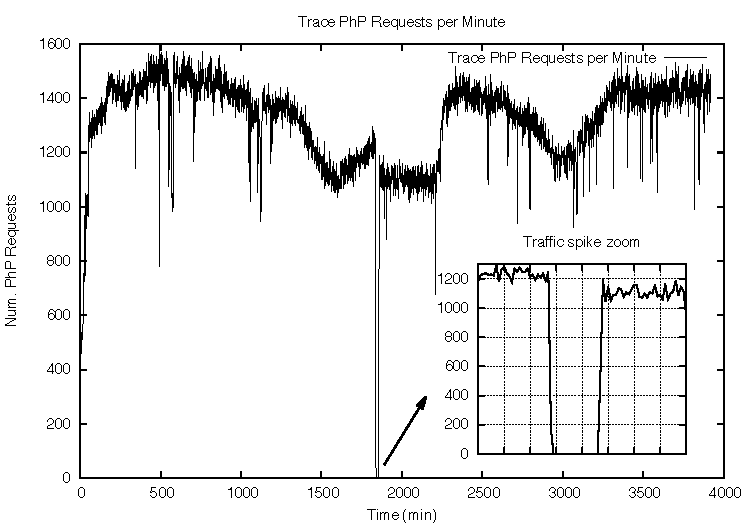
\includegraphics[width=0.49\textwidth, height=6cm]{./images/traceWorkload_zoom}
\end{center}
\vspace{-5mm}
\caption{Wikipedia trace workload.}
\label{workload}
\end{figure}




%\fixme{Change the textcolor for the medium vm instances.}


\subsection{Public Cloud}

Initially, our experiments on EC2 used small instances for the PHP service and one large instance for the MySQL service. Table~\ref{EC2instances} details the hardware configuration and cost per-hour of the different sizes of EC2 instances employed during the experiments.




\subsubsection{Performance stability and SLO fulfillment} 
Figure~\ref{fig:EC2ResponseTime} represents the degree of SLO fulfillment of three different classes of customers, indicating the response time data-points obtained during the execution of the Wikipedia workload trace. In particular, Figure~\ref{fig:EC2ResponseTime} focus on the interval of time in which the outage occurred. The results show how the system scales back when the request volume drops, and quickly scales in when the load increases suddenly. As shown on Figure~\ref{fig:EC2ResponseTime},  the degree of SLO fulfillment gradually improves depending on the tradeoff performance/cost of each customer chosen to handle this traffic anomaly. Thus, the \emph{bronze} and \emph{silver} customers employ between 150 and 200 minutes to reach the performance stability,  but experiencing more SLO violations when using a \emph{bronze} customer. While the \emph{gold} customer requires less time to handle this traffic spike reducing at the maximum the number of violations, as detailed in Table~\ref{summaryEC2}. The selection of different performance/cost configurations, and consequently different classes of customer, has important consequences, specially when a non-fulfillment of the requirements affects to the revenues of the customer.

\begin{figure*}[htb]
	\begin{minipage}[b]{0.32\linewidth}
		\captionof*{figure}{{\scriptsize \textbf{Bronze}}}
		\vspace{-4mm}
		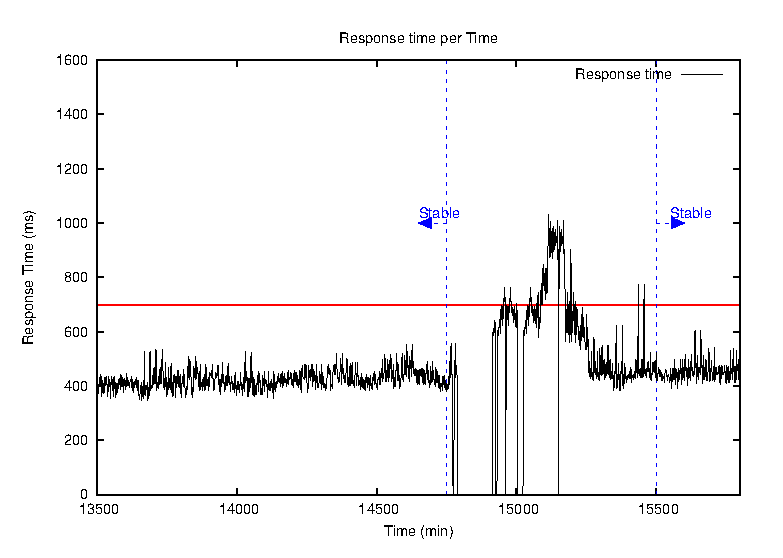
\includegraphics[height=4cm]{images/exps2011/low/ec2/proxyDataPoints_output_filtered.eps}	
		\vspace{-4mm}
	\end{minipage}
	\hfill
	\begin{minipage}[b]{0.32\linewidth}
		\captionof*{figure}{{\scriptsize \textbf{Silver}}}
		\vspace{-4mm}
		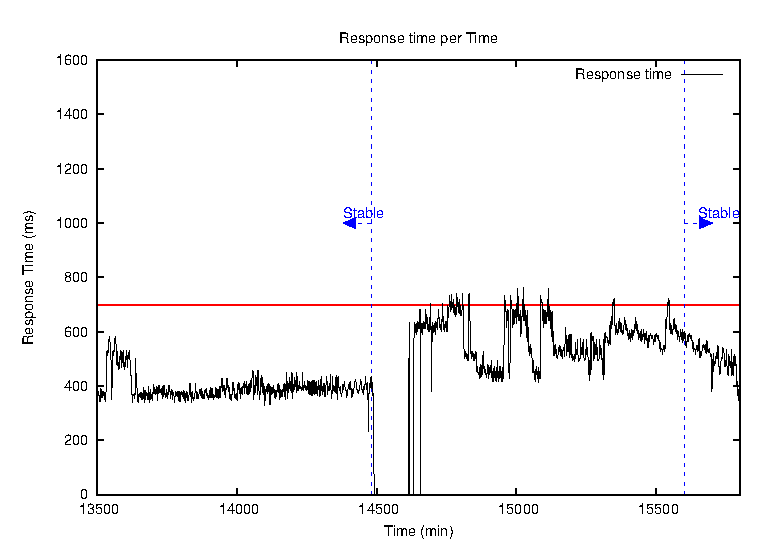
\includegraphics[height=4cm]{images/exps2011/medium/ec2/proxyDataPoints_output_filtered.eps}
		\vspace{-4mm}
	\end{minipage}
\hfill
\begin{minipage}[b]{0.32\linewidth}
		\captionof*{figure}{{\scriptsize \textbf{Gold}}}
		\vspace{-4mm}
		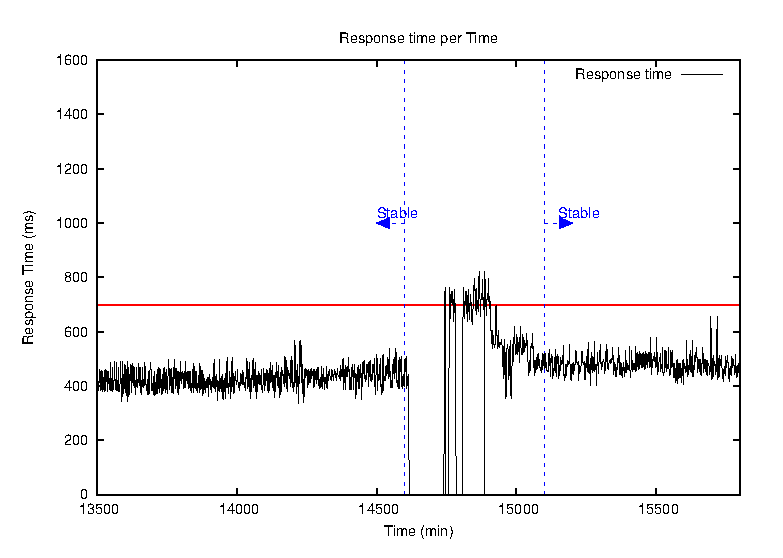
\includegraphics[height=4cm]{images/exps2011/high/ec2/proxyDataPoints_output_filtered.eps}
		\vspace{-4mm}
	\end{minipage}
\caption{EC2: Response time values during the outage.}
\label{fig:EC2ResponseTime}
\end{figure*}


\subsubsection{Resource utilization} 
To better understand the impact of selecting a scaling plan adapted to the customer preferences, we shall also focus on the resource consumption illustrated on Figure~\ref{fig:EC2Instances}. While satisfying the requirements, the allocation of poor hardware configurations can easily expose the system to performance degradations, and consequently increases the time required to stabilize the system performance. This can be seen on  Figure~\ref{fig:EC2Instances}(left), in the time interval between t=338min and t=400min. The \emph{bronze} customer provisions a low-cost configuration, that compromises the performance and raises an important amount of SLO violations during a long period of time. Unlike the \emph{silver} and \emph{gold} customer utilizes along the whole execution powerful configurations that enables to minimize these degradations. Specifically, the \emph{gold} customer allocates a costly resource combination (mainly composed of \emph{m1.large} instance types) which is able to handle such traffic changes while avoiding the under-utilization of the resources. This lack of under-utilization can be depicted in Figure~\ref{fig:EC2ResponseTime}, where the processing time remains close to the SLO after the new scaling plan is provisioned.

%The system's unstability is clearly shown in the planB where the resource combination changes from 1800-2000m till find an optimal resource combination to handle the traffic.

\begin{figure*}[htb]
	\begin{minipage}[b]{0.32\linewidth}
		\captionof*{figure}{{\scriptsize \textbf{Bronze}}}
		\vspace{-4mm}
		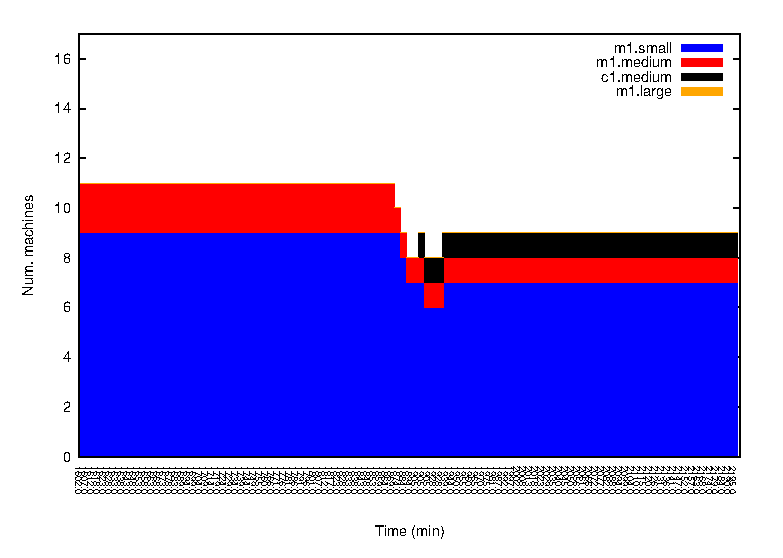
\includegraphics[height=4cm]{images/exps2011/low/ec2/inst_type_machines_filtered.eps}	
		\vspace{-4mm}
	\end{minipage}
	\hfill
	\begin{minipage}[b]{0.32\linewidth}
		\captionof*{figure}{{\scriptsize \textbf{Silver}}}
		\vspace{-4mm}
		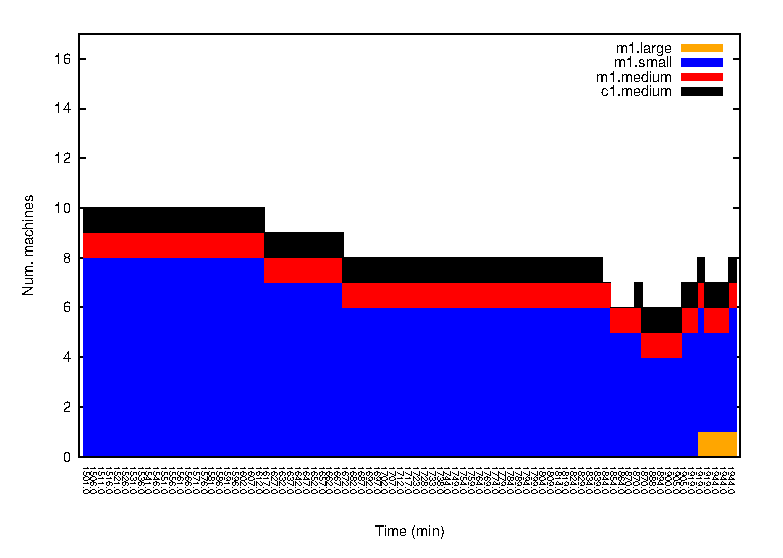
\includegraphics[height=4cm]{images/exps2011/medium/ec2/inst_type_machines_filtered.eps}
		\vspace{-4mm}
	\end{minipage}
\hfill
\begin{minipage}[b]{0.32\linewidth}
		\captionof*{figure}{{\scriptsize \textbf{Gold}}}
		\vspace{-4mm}
		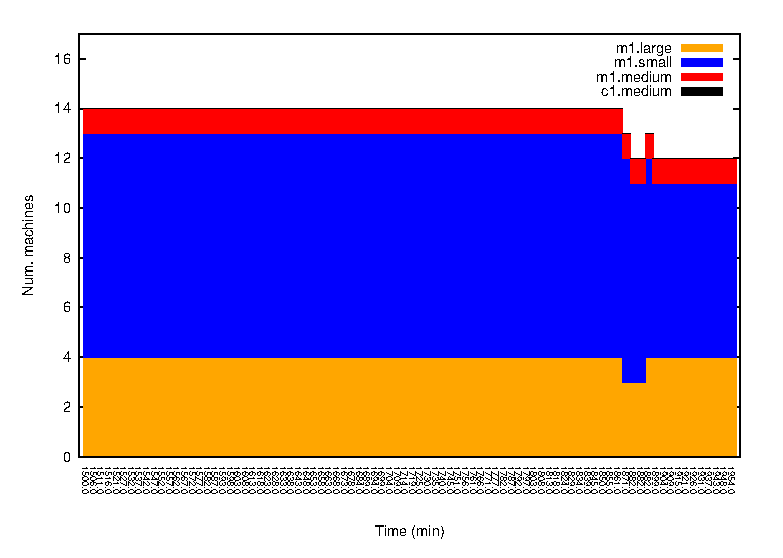
\includegraphics[height=4cm]{images/exps2011/high/ec2/inst_type_machines_filtered.eps}
		\vspace{-4mm}
	\end{minipage}
\caption{EC2: Cloud instances provisioned to handle the outage.}
\label{fig:EC2Instances}
\end{figure*}

\subsubsection{Analysis of results}
The results of the three runs are summarized in Table~\ref{summaryEC2}, where we show the amount of SLO violations, the number of provisioning decisions taken by the autoscaling system and an estimation of the cost of running the VMs in Amazon EC2.

As depicted on Figure~\ref{fig:EC2ResponseTime} and Figure~\ref{fig:EC2Instances}, the selection of one hardware configuration or another has a direct effect in the performance. The use of \emph{bronze} settings shows the vulnerability of selecting a configuration with low operational cost, as it easily becomes unstable when handling bursty workloads. Hence, poor hardware configurations increase the probability of experiencing SLO violations under sudden traffic spikes, outages or other traffic anomalies. 

When using a mixed configuration like \emph{silver}, the \emph{Scaler} explores the tradeoff between performance capacity and cost by combining different hardware configurations to handle the load with an acceptable cost. However, the discovery of such resource combination can be hard-to-find, affecting to the stability of the application due to frequent scaling actions, as shown on Figure~\ref{fig:EC2ResponseTime}(center). Finally, with a \emph{gold} customer, the Scaler provisions resources that offer better performance in exchange for a higher infrastructure cost. With little over-provisioning, this class of customer configuration enforces the QoS requirements and improves considerably the stability and performance of the system by distributing the new request volume across the most powerful resources.  

Note that due to synchronization time lag between the scaling actions and the displayed information in the logs, time values are shifted for a few minutes during the whole execution, as shown in Figure~\ref{fig:EC2Instances} and Figure~\ref{fig:EC2ResponseTime}.


%Another interesting aspect that we noticed during these experiments is the economical impact of selecting one class of customer or another when minimizing the SLO violations.

%\fixme{Include a plot showing the infra cost vs penalty cost for a bronze customer}
%\fixme{The unstability of silver EC2 is also provoked in some part due to the load balancing system which have to adapt the weights to a wide number of different types of resoruces.}


 %This type of provisioning decisions enable to handle these traffic anomalies by distributing the new request volume across the most powerful resources. 


%\vspace{3mm}
%\noindent\textbf{SLO violation cost VS Infrastructure cost:}

%\begin{figure*}[htb]
%	\begin{minipage}[b]{0.32\linewidth}
%		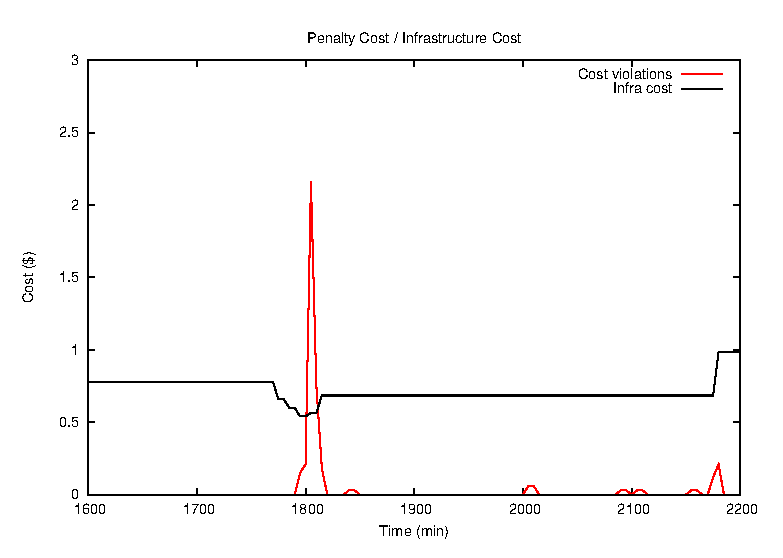
\includegraphics[height=4cm]{images/exps2011/low/ec2/penaltyVScost_filtered.eps}	
%		\vspace{-4mm}
%	\end{minipage}
%	\hfill
%	\begin{minipage}[b]{0.32\linewidth}
%		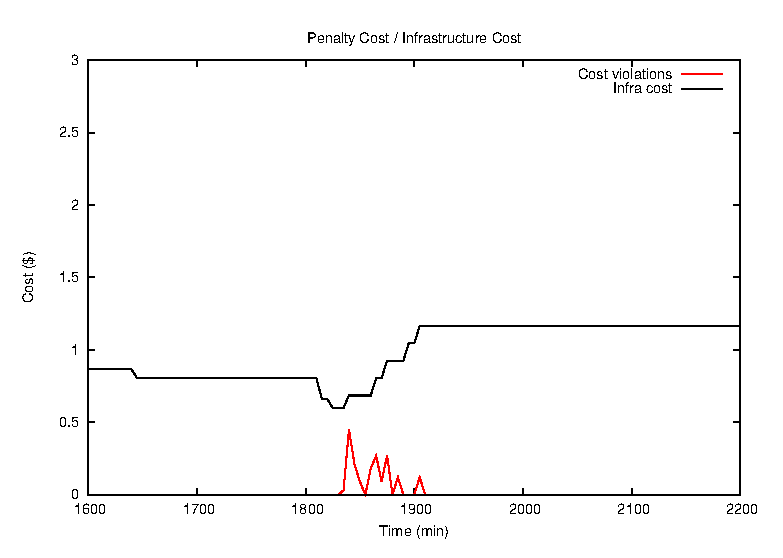
\includegraphics[height=4cm]{images/exps2011/medium/ec2/penaltyVScost_filtered.eps}
%		\vspace{-4mm}
%	\end{minipage}
%\hfill
%\begin{minipage}[b]{0.32\linewidth}
%		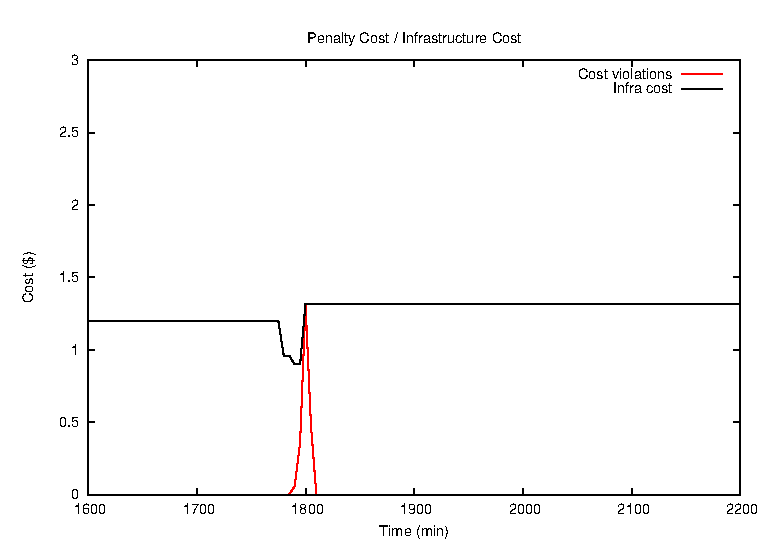
\includegraphics[height=4cm]{images/exps2011/high/ec2/penaltyVScost_filtered.eps}
%		\vspace{-4mm}
%	\end{minipage}
%\caption{Cloud instances provisioned to handle the outage.}
%\label{fig:EC2Penalty}
%\end{figure*}


\begin{table}
  {\scriptsize 
\begin{center}
    \begin{tabular}{  | c | c | c | c |}
    \hline
         \textbf{Customer}  & \textbf{SLO Violations} & \textbf{Decisions}  & \textbf{Cost}  \\ \hline
   \textit{Bronze}   &  117 &  6 &  6.9 \$ \\ \hline   
   \textit{Silver}  &  74 &  14 &  8,6 \$ \\ \hline   
\textit{Gold} &   63  &  4 &  10.8 \$  \\ \hline   

 \end{tabular}
\end{center}
\vspace{-5mm}
\caption{Analysis of results on EC2}
\label{summaryEC2}
}
\end{table}




%%% EXPERIMENTS DAS4 %%%%


\subsection{Private Cloud}

Our experiments on DAS-4 rely on OpenNebula as IaaS~\cite{sotomayor_virtual_2009}. To deploy the Wikipedia services, we initially provisioned \emph{small} instances for the PHP service and one \emph{large} instance for the MySQL service. Additionally, for these experiments, we specified a cost per-hour for each one of the available resources, and extended from three to five the initial customer classification: \emph{platinum, gold, silver, bronze} and \emph{copper}. Table~\ref{DAS4instances} detailed the hardware configurations of the different VM sizes in DAS-4.

%following the same criteria of SLO fulfillment and infrastructure cost



%\subsubsection{Performance impact of the outage}
\subsubsection{Performance stability and SLO fulfillment}

Figure~\ref{fig:DAS4ResponseTime} shows the performance behavior of the scaling plans selected for five types of customers. As depicted in Figure~\ref{fig:DAS4ResponseTime}, the performance stability is mainly affected by two aspects: frequent scalings operations and traffic spikes. Thus, the \emph{platinum} customer presents an unstable performance pattern, due to numerous provisioning actions aiming to find the optimal scaling plan. In contrast, the performance behavior of the \emph{gold} customer shows no oscillations even during the outage, which can be explained by the selection of an appropriate resource combination that do not under-utilizes the resources.

%an optimal combination of resources that stabilizes the performance even during the outage. 


Regarding the traffic spikes caused by the new workload, it is clear how customer configurations, like \emph{copper, bronze and silver}, are vulnerable to traffic changes, thus causing SLO violations. As shown on Figure~\ref{fig:DAS4ResponseTime},  the scaling decisions that prioritizes the infrastructure cost than performance are directly affected by the effects of the request volume increment. This can be seen in the time interval between t=510min and t=536min for the \emph{copper} customer, and between t=498min and t=519min for the \emph{bronze} customer, respectively. By selecting an appropriate scaling plan, the performance stability and SLO fulfillment can be better enforced without dramatically raising the cost.

%In this case, the combination of one highcpu-medium and two small vm instances were enough to handle the new request volume without causing SLO violations.

%On the other hand, when using the copper and bronze configurations, the system becomes vulnerable to traffic fluctuations. In this case, it can be seen in the interval of time t=ms and t=ms for the copper and bronze customers.




\begin{figure*}[htb]
	\begin{minipage}[b]{0.20\linewidth}
		\captionof*{figure}{{\scriptsize \textbf{Copper}}}
		\vspace{-4mm}
		\includegraphics[width=\linewidth,height=4cm]{images/exps2011/low/das/proxyDataPoints_output.eps}	
		\vspace{-4mm}
	\end{minipage}
	\hfill
\begin{minipage}[b]{0.19\linewidth}
		\captionof*{figure}{{\scriptsize \textbf{Bronze}}}
		\vspace{-4mm}
		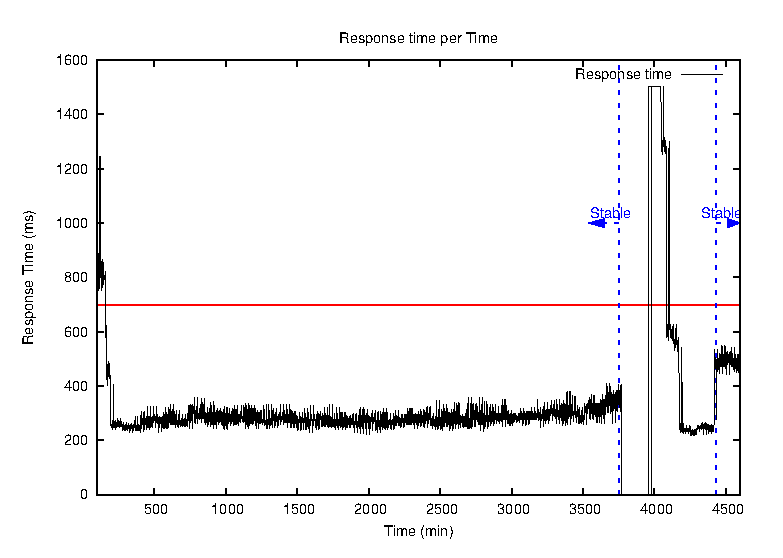
\includegraphics[width=\linewidth,height=4cm]{images/exps2011/medium_down/das/proxyDataPoints_output.eps}
		\vspace{-4mm}
	\end{minipage}
\hfill
	\begin{minipage}[b]{0.2\linewidth}
		\captionof*{figure}{{\scriptsize \textbf{Silver}}}
		\vspace{-4mm}
		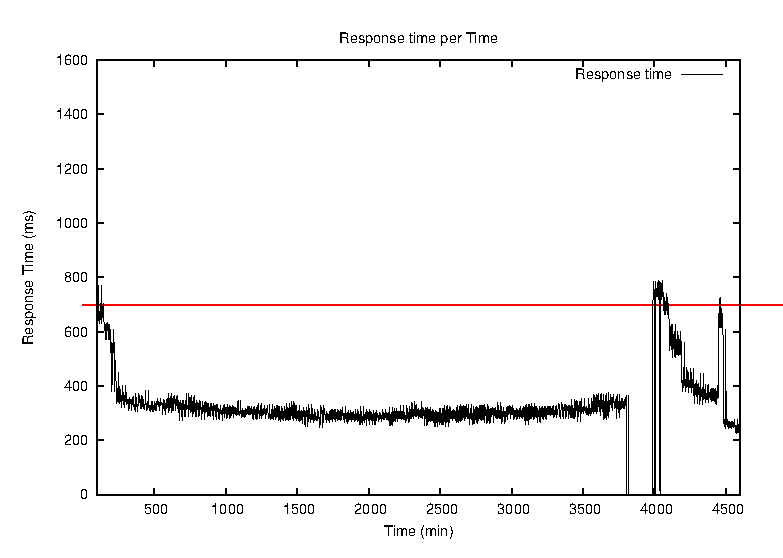
\includegraphics[width=\linewidth,height=4cm]{images/exps2011/medium/das/proxyDataPoints_output.eps}
		\vspace{-4mm}
	\end{minipage}
\hfill
\begin{minipage}[b]{0.2\linewidth}
		\captionof*{figure}{{\scriptsize \textbf{Gold}}}
		\vspace{-4mm}
		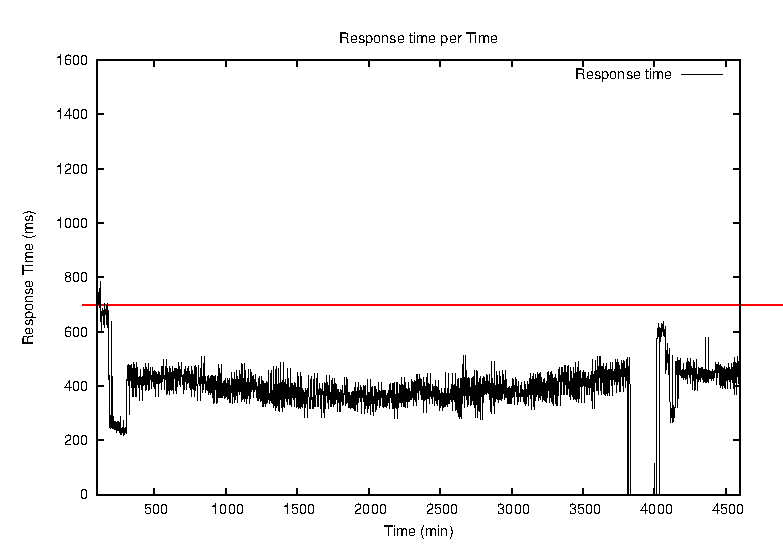
\includegraphics[width=\linewidth,height=4cm]{images/exps2011/medium_up/das/proxyDataPoints_output.eps}
		\vspace{-4mm}
	\end{minipage}
\hfill
\begin{minipage}[b]{0.19\linewidth}
		\captionof*{figure}{{\scriptsize \textbf{Platinum}}}
		\vspace{-4mm}
		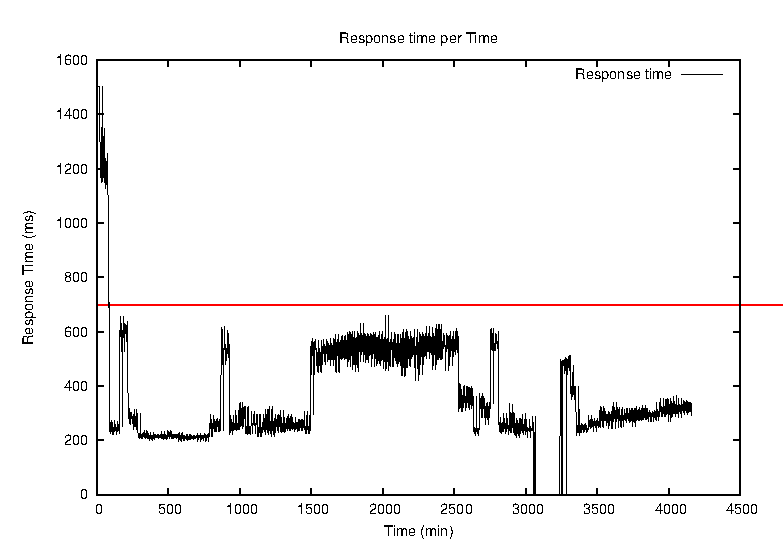
\includegraphics[width=\linewidth,height=4cm]{images/exps2011/high/das/proxyDataPoints_output.eps}
		\vspace{-4mm}
	\end{minipage}
\caption{DAS4: Response time values during the outage.}
\label{fig:DAS4ResponseTime}
\end{figure*}


\subsubsection{Resource utilization}

As explained above, frequent scaling actions can affect to the performance stability, but also inappropriate scaling decisions. This can be seen in Figure~\ref{fig:DAS4Instances}, where the \emph{copper} and \emph{bronze} customers attempt to scale back the system when the load drops, but the resulting resource combinations cannot handle the new request volume, and the system is scaled up again.  At difference, the \emph{gold} customer only de-provisions low-powered resources during the outage, which enables to distribute the new load among the current resources, while new resources are allocated to avoid future resource over-utilization. 

Once the outage occurred, another interesting aspect to notice is the type of resources employed to minimize the number of SLO violations. While the \emph{silver} customer provisions powerful machines (e.g. \emph{highcpu-medium}) that quickly mitigate the degradations, the \emph{copper} customer allocates \emph{small} resources that employ more time to handle the workload. When using the \emph{gold} or \emph{platinum} settings, the system barely appreciates the changes in the workload, as shown on Figure~\ref{fig:DAS4ResponseTime}. It demonstrates the importance of using autoscaling system that exploits the resource heterogeneity of cloud infrastructures to satisfy customer preferences.

% thus justifying the use of different sizes of resources to better enforce the QoS requirements. 

On the other hand, it is remarkable to point out that the amount of allocated resources may not be a subject of comparison between customer configurations. The poor performance isolation and the variable network bandwidth can affect to the performance of the resources, and consequently the amount of allocated resources can vary even for the same customer.


%In this case, the combination of one highcpu-medium and two small vm instances were enough to handle the new request volume without causing SLO violations.


\begin{figure*}[htb]
	\begin{minipage}[b]{0.19\linewidth}
		\captionof*{figure}{{\scriptsize \textbf{Copper}}}
		\vspace{-4mm}
		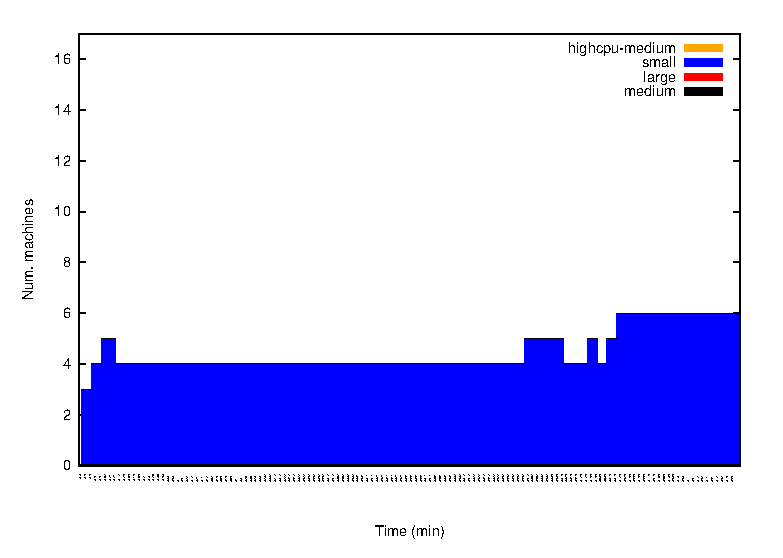
\includegraphics[width=\linewidth,height=4cm]{images/exps2011/low/das/inst_type_machines.eps}	
		\vspace{-4mm}
	\end{minipage}
	\hfill
\begin{minipage}[b]{0.2\linewidth}
		\captionof*{figure}{{\scriptsize \textbf{Bronze}}}
		\vspace{-4mm}
		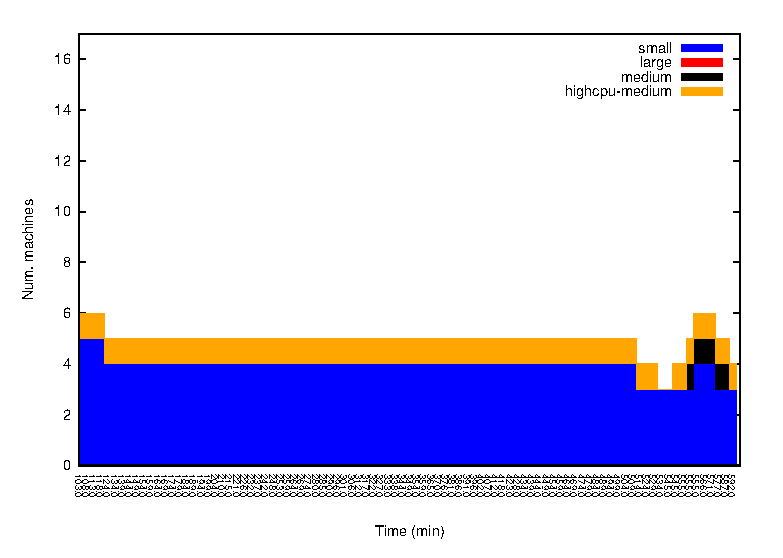
\includegraphics[width=\linewidth,height=4cm]{images/exps2011/medium_down/das/inst_type_machines.eps}
		\vspace{-4mm}
	\end{minipage}
\hfill
	\begin{minipage}[b]{0.2\linewidth}
		\captionof*{figure}{{\scriptsize \textbf{Silver}}}
		\vspace{-4mm}
		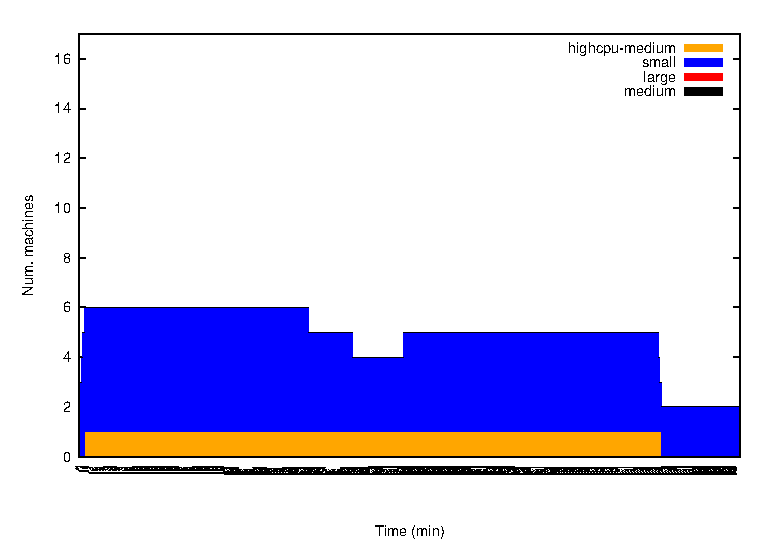
\includegraphics[width=\linewidth,height=4cm]{images/exps2011/medium/das/inst_type_machines.eps}
		\vspace{-4mm}
	\end{minipage}
\hfill
	\begin{minipage}[b]{0.2\linewidth}
		\captionof*{figure}{{\scriptsize \textbf{Gold}}}
		\vspace{-4mm}
		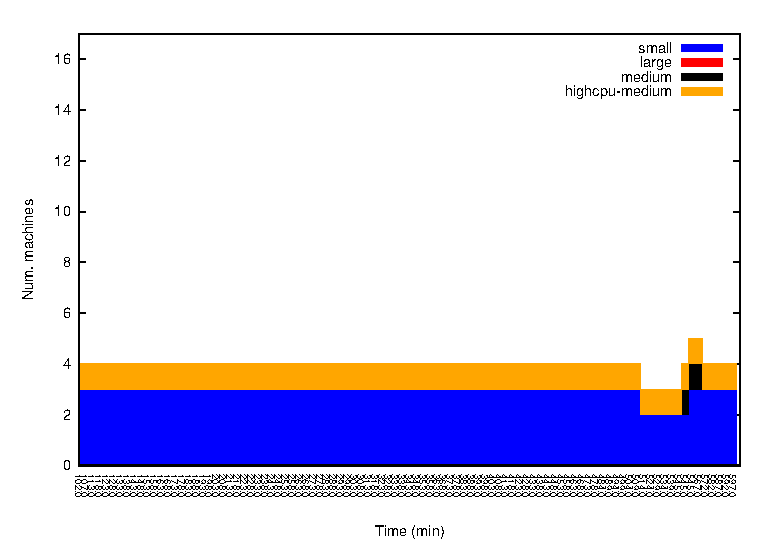
\includegraphics[width=\linewidth,height=4cm]{images/exps2011/medium_up/das/inst_type_machines.eps}
		\vspace{-4mm}
	\end{minipage}
\hfill
\begin{minipage}[b]{0.19\linewidth}
		\captionof*{figure}{{\scriptsize \textbf{Platinum}}}
		\vspace{-4mm}
		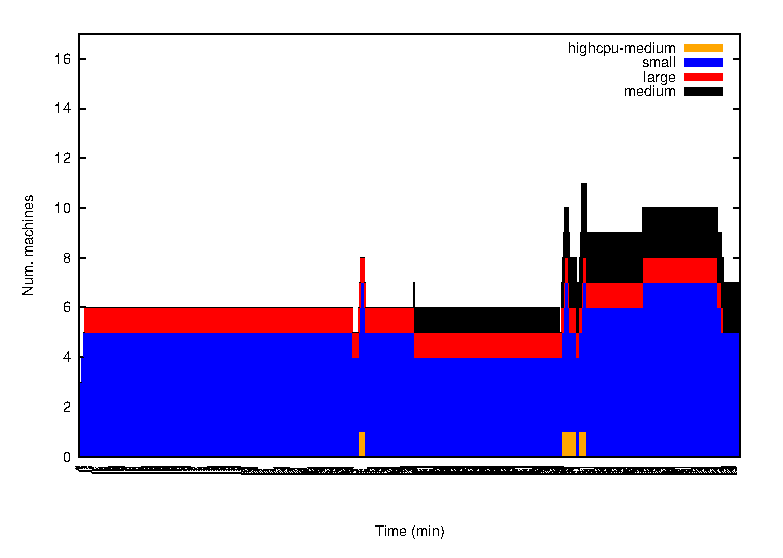
\includegraphics[width=\linewidth,height=4cm]{images/exps2011/high/das/inst_type_machines.eps}
		\vspace{-4mm}
	\end{minipage}
\caption{DAS4: Cloud instances provisioned to handle the outage.}
\label{fig:DAS4Instances}
\end{figure*}

%\paragraph{SLO violation cost VS Infrastructure cost}

%\begin{figure*}[htb]
%	\begin{minipage}[b]{0.32\linewidth}
%		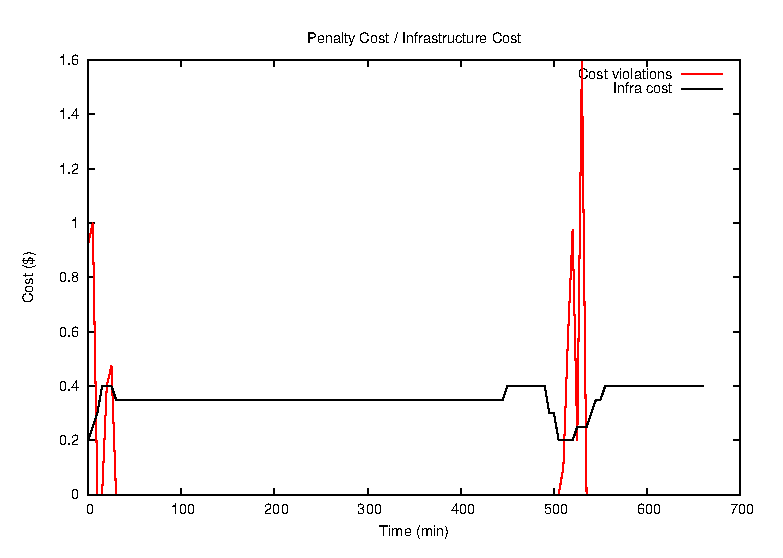
\includegraphics[height=4cm]{images/exps2011/low/das/penaltyVScost.eps}	
%		\vspace{-4mm}
%	\end{minipage}
%	\hfill
%	\begin{minipage}[b]{0.32\linewidth}
%		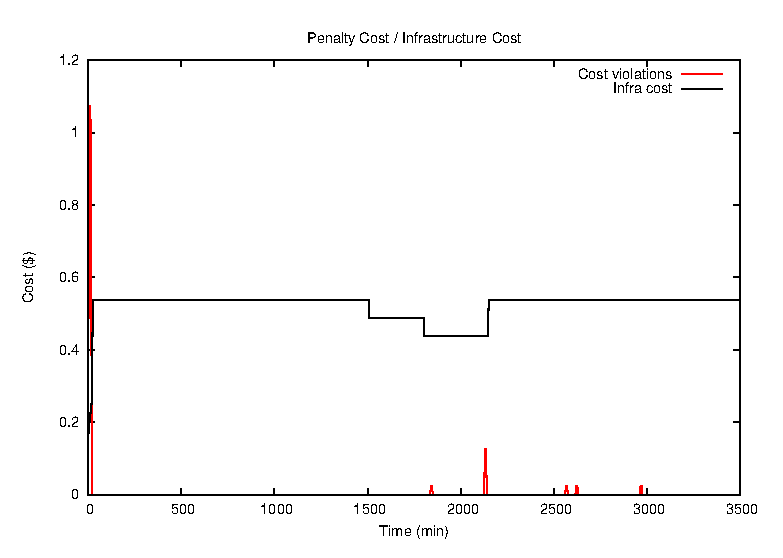
\includegraphics[height=4cm]{images/exps2011/medium/das/penaltyVScost.eps}
%		\vspace{-4mm}
%	\end{minipage}
%\hfill
%\begin{minipage}[b]{0.32\linewidth}
%		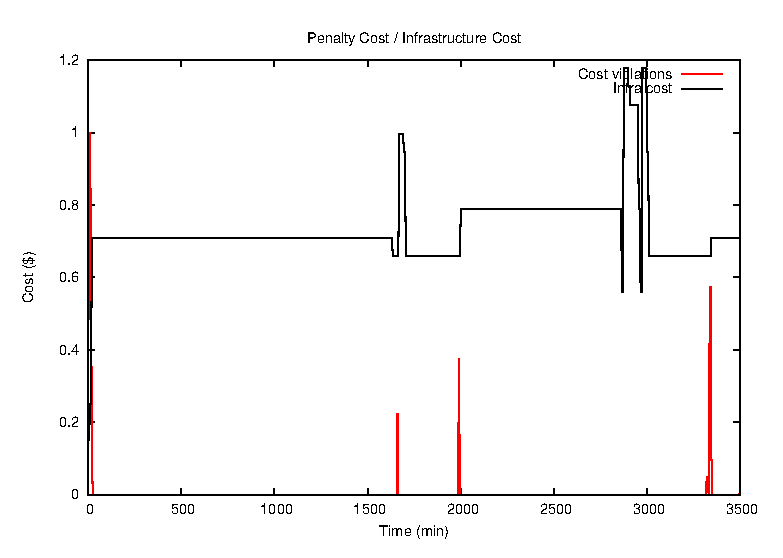
\includegraphics[height=4cm]{images/exps2011/high/das/penaltyVScost.eps}
%		\vspace{-4mm}
%	\end{minipage}
%\caption{Cloud instances provisioned to handle the outage.}
%\label{fig:DASPenalty}
%\end{figure*}

\begin{table}
  {\scriptsize 
\begin{center}
    \begin{tabular}{  | c | c | c | c  |}
    \hline
         \textbf{Customer}  & \textbf{SLO Violations} & \textbf{Decisions}  & \textbf{Cost}   \\ \hline
   \textit{copper}   & 138  &  6 &  6.4 \$ \\ \hline   
   \textit{bronze}  &  129 &   8&  9.5 \$  \\ \hline   
   \textit{silver}  &  82  & 10  &  10.4 \$  \\ \hline   
   \textit{gold}  & 0  &  4  &   8.3 \$    \\ \hline   
\textit{platinum} &  0 & 24 & 12.8 \$  \\ \hline   

 \end{tabular}
\end{center}
\vspace{-5mm}
\caption{Analysis of results on DAS4}
\label{summaryDAS4}
}
\end{table}

\subsubsection{Analysis of results}

Table~\ref{summaryDAS4} summarizes the results of these experiments, where we show the amount of SLO violations, provisioning decisions and total infrastructure cost of the allocated resources. 

Firstly, we noticed a progressive minimization of the SLO violations related to the class of customer, and therefore due to the hardware configuration provisioned at the moment of the traffic increased. During the outage, the \emph{copper} and \emph{bronze} customers used poor hardware configurations which were unabled to handle the new workload. In contrast, the \emph{gold}  and \emph{platinum} customers allocated powerful and suited resources that handled the new load successfully.

Secondly, it is remarkable how depending of the scaling plan the required time to stabilize the system vary, and as a consequence the amount of SLO violations. An explanation comes from the quickly allocation of powerful resources, instead of a gradual allocation of standard or less-powered resources. This decision has special importance in cloud platforms aiming to reduce the penalties paid due to SLO violations or server errors. For instance, RackSpace~\cite{rackspace} guarantees 100\% availability of the hosted services, with a penalty equal to 5\% of the fees for each 30 minutes of network or data center downtime. Therefore, the minimization of the penalties affects to the revenues but also to the user base.

Finally, we also note some performance unstability with the \emph{platinum} customer that was provoked in some situations due to wrong or delay balancing of the incoming traffic across the heterogeneous resources.

Note that due to synchronization time lag between the scaling actions and the displayed information in the logs, time values shown in Figure~\ref{fig:DAS4Instances} and Figure~\ref{fig:DAS4ResponseTime} are shifted for a few minutes during the whole execution.

